\chapter{Koji DNK šabloni igraju ulogu molekularnog sata?}
\section{Biološki problem}

Bioritam svih živih bića kotroliše ‚‚unutrašnji časovnik'' koji još zovemo i cirkadijalni. Ljudi koji često putuju avionom na drugi kraj sveta mogu to da osete kada pokušaju da zaspe nakon promene nekoliko vremenskih zona. Kao i svaki sat, i ovaj može da se pokvari, što rezultuje genetskom bolešću pod nazivom sindrom odložene faze spavanja. Njegova osnova je na molekularnom nivou. Mnogi procesi su kontrolisani ovim časovnikom, što ilustruje slika 2.1. Kao što vidimo, postoji tačno određeno vreme u toku dana kada telo ima najnižu temperaturu, kada kreće i prestaje lučenje hormona poput melatonina (neophodnog za kvalitetan san) i slično.

\iffalse 
\begin{figure}[h]
\centering
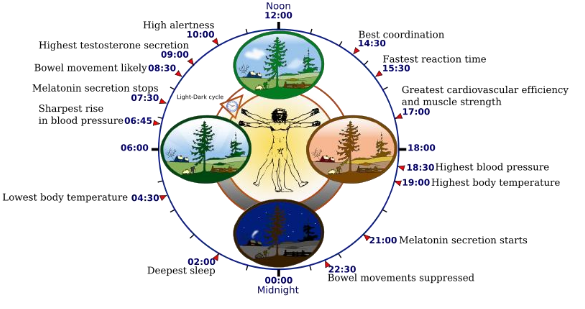
\includegraphics[width=1.1\textwidth]{poglavlja/2/slike/12cut.PNG}
\caption{Cirkadijalni ritam}
\end{figure}
\fi 

Naučnici su se pitali kako ćelije znaju kada treba da uspore ili ubrzaju proizvodnju određenih proteina. Ranih sedamdesetih, Ron Konopka i Sejmor Benzer su napravili prve korake ka rešavanju ove misterije. Do danas je otkriveno mnogo cirkadijalnih gena koji koordiniraju ponašanje stotine drugih gena. \\
\indent Kod čoveka, cirkadijalni ritam je promenljiv, tj. varira od osobe do osobe. Mi ćemo se u daljem tekstu fokusirati na biljke, jer je kod njih cirkadijalni ritam pitanje života i smrti, stoga ne sme biti promenljiv. Geni biljaka moraju znati kada sunce izlazi i zalazi kako bi znali kada treba vršiti fotosintezu, jer je ona od krucijalne važnosti za život biljke, a usko povezana sa količinom sunčeve svetlosti. Primeri specifičnih ponašanja nekih biljaka u zavisnosti od cirkadijalnog ritma dati su na slici 2.2.

\iffalse 
\begin{figure}[!htb]\centering
    \caption{Cirkadijalni ritam biljke}
   \begin{minipage}{0.5\textwidth}
     \frame{
\includegraphics[width=.7\linewidth]{poglavlja/2/slike/13-1.PNG}}
   \end{minipage}
   \begin {minipage}{0.4\textwidth}
     \frame{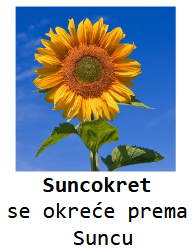
\includegraphics[width=.7\linewidth]{poglavlja/2/slike/13-2.PNG}}
   \end{minipage}
\end{figure}
\fi 

Ispostavlja se da svaka ćelija biljke čuva podatak o tome da li je dan ili noć nezavisno od drugih ćelija, kao i da su samo tri gena odgovorna za upravljanje satom. Oni kodiraju regulatorne proteine (transkripcione faktore)- to su LCY, CCA1 i TOC1. Spoljašnji faktori, kao što je količina sunčeve svetlosti, kontrolišu regulatorne gene i regulatorne proteine kako bi organizmi prilagodili svoju gensku ekspresiju, odnosno da li će se protein sintetisati u to vreme ili ne. Dakle, svaki metabolički proces je regulisan cirkadijalnim časovnikom kojim upravljaju regulatorni proteini, odlučujući kada će se koji protein u ćeliji biljke sintetisati. Regulatorni proteini upravljaju genskom ekspresijom tako što se vežu za DNK u trenucima kada je potrebno sintetisati neki protein važan za cirkadijalni ritam, kao što je prikazano na slici 2.3. Naravno, to vezivanje se ne može ostvariti bilo gde u okviru DNK, već postoje posebna mesta, kao što je prikazano na slici 2.4. Ta posebnost je neophodna iz više razloga. Regulatorni protein mora znati gde treba da se veže, a isto tako DNK mora znati kako da to protumači, odnosno, to za nju mora biti signal da je vreme započeti sintezu, kao i pružiti informaciju o kom se proteinu radi. Ta posebna mesta predstavljaju manje skupove nukleotida u DNK koji nazivamo \textbf{regulatorni motivi}. Naš zadatak je da ih pronađemo. 

\iffalse 
\begin{figure}[h]
\caption{Regulatorni proteini na delu}
\centering
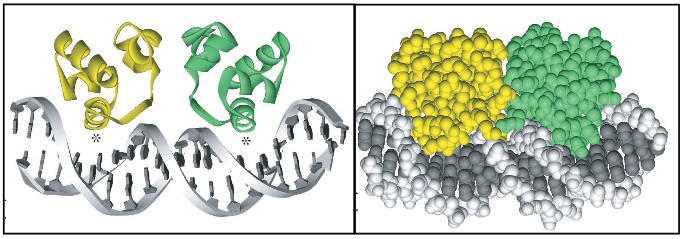
\includegraphics[width=0.55\textwidth]{poglavlja/2/slike/14.PNG}
\end{figure}
\fi 

\begin{figure}[h]
\caption{Mesta vezivanja regulatornih proteina}
\centering
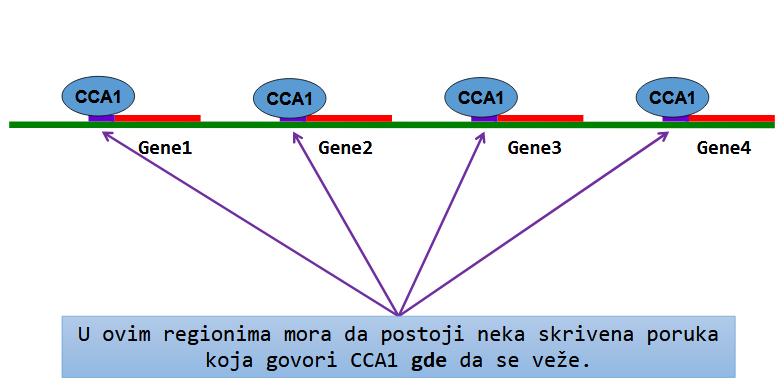
\includegraphics[width=0.7\textwidth]{poglavlja/2/slike/16.PNG}
\end{figure}


\section{Informatički problem}

Kako bismo informatički rešili problem pronalaženja regulatornih motiva u DNK, moramo predstaviti sve gorepomenute biološke pojmove na način koji bi informatičar i njegov računar mogli razumeti i obraditi. 

\begin{itemize}
    \item Iz ove tačke gledišta, DNK predstavlja nisku karaktera nad azbukom: {A, G, T, C}.
    \item Kodirajuće sekcije DNK (one koje se prepisuju i prevode u proteine) za nas će biti podniske niske DNK.
    \item Regulatorni motiv je šablon koji se pojavljuje tačno jednom u svakoj kodirajućoj sekciji DNK.
\end{itemize}

Hajde da damo u računarskom smislu korektnu definiciju problema: \\
\begin{tcolorbox}
\textbf{Informatička definicija problema nalaženja regulatornih motiva u DNK} \\
\textbf{Ulaz:} N niski koje predstavljaju kodirajuće sekvence DNK.\\
\textbf{Izlaz:} Podniska dužine k koja predstavlja regulatorni motiv (skrivenu poruku, mesto vezivanja regulatornih proteina).
\end{tcolorbox} 

Ovaj problem nas podseća na problem pronalaženja \textit{OriC}-a, koji smo rešavali svodeći ga na pronalaženje čestih reči u tekstu koristeći algoritam \textit{FrequentWords}, detaljno opisan u prethodnom poglavlju. Da bismo taj algoritam primenili ovde, neophodno je da od niza niski dobijemo konkatenacijom jednu veliku nisku, na koju ćemo primeniti ovaj algoritam. \\

Međutim, ovaj algoritam nije primenljiv ako motivi mutiraju. Možemo pokušati da primenimo algoritam \textit{FrequentWordsWithMissmatches}. To bi nas dovelo do tačnog rešenja, ali nakon previše vremena. Naime, kada smo nalazili \textit{OriC}, tražili smo uzorke dužine 9 karaktera (DnaA box je bio te dužine). U ovom slučaju, tražimo motive koji su najčešće dužine 15 karaktera, pa nam ovaj algoritam ne radi dovoljno brzo. Dakle, potrebna nam je nova ideja. 

\section{Problem ubačenog motiva}

I dalje pokušavamo da pronađemo skrivenu poruku u DNK koja kodira mesto vezivanja regulatornih proteina za DNK. Dali smo korektnu definiciju problema i, kao pravi matematičari, pokušali najpre da svedemo problem na neki drugi, koji smo već rešili. Međutim, to nas je odvelo u veliku vremensku složenost, pa samim tim i neupotrebljivost pronađenog algoritma za rešavanje. Zaključili smo da nam je potreban novi pristup, tj. da moramo probati da problem rešimo direktno - bez pomoći algoritama za \textit{OriC}. Za ovako nešto, neophodno je najpre definisati još nekoliko pojmova vezanih za šablone koje pokušavamo da pronađemo:

\begin{itemize}
    \item Mutirani šablon predstavlja šablon u kome se na nekim mestima može pojaviti mutacija, odnosno odstupanje od početne niske.
    \item $(k, d)$ motiv je k-gram koji se pojavljuje u svakoj sekvenci sa najviše $d$ razlika.
    \item Kanonski motiv predstavlja motiv koji tražimo (bez uticaja mutacija).
    \item Instance su mutirani motivi - oni koji se pojavljuju u niskama sa najviše $d$ grešaka, odnosno razlika u odnosu na kanonski motiv.
\end{itemize}

Sada, kada smo tačno i precizno definisali pojmove koji će nam igrati uloge regulatornih motiva, izmenićemo i samu definiciju problema, tj. malo promeniti scenario tako da se sve uloge lepo uklope, pazeći naravno da ne izgubimo na tačnosti definicije.

\begin{tcolorbox}
\textbf{Problem ubačenog motiva:} Pronalaženje $(k, d)$ motiva u skupu niski\\
\textbf{Ulaz:} Skup niski $Dna$ i celi brojevi $k$ (dužina motiva) i $d$ (maksimalni broj razlika).\\
\textbf{Izlaz:} Svi $(k, d)$ motivi u skupu $Dna$.
\end{tcolorbox}

Nova definicija problema izrodiće nekoliko novih ideja za njegovo rešavanje, a te ideje izrodiće nove algoritme. U daljem tekstu prikazaćemo nekoliko rešenja, uz osvrt na ideju koja nas je do njega dovela.


\subsection{Enumeracija motiva}
Početna ideja je zasnovana na gruboj sili - za svaki k-gram ćemo ispitati da li je $(k, d)$ motiv za dati skup niski. Dakle, trebalo bi generisati $4^k$ kombinacija i za svaku ispitati da li je $(k, d)$ motiv. Postavlja se pitanje da li je potrebno ispitati svih $4^k$ kandidata. 

\noindent Pogledajmo na primer sledeći skup niski:
$$\textbf{AAATTTAAATTTAAATTT}$$ 
$$\textbf{TTTAAATTTAAATTTAAA}$$
Da li ima smisla proveravati 8-gram GGAAGGAA?
Naravno da nema! Karakter G se ne pojavljuje ni u jednoj niski iz našeg skupa.
Zato sigurno ne može biti traženi $(k,d)$ motiv.
Dakle, prvo možemo izbaciti kandidate koji se ne pojavljuju ni u jednoj niski iz skupa $Dna$.
Takođe, možemo primetiti da je skup instanci jednog kandidata koje se pojavljuju u ostalim niskama (ceo skup $Dna$, bez niske u kojoj je dati kandidat podniska) prilično ograničen. Ograničenje nameće broj $d$. Dakle, jasno je da treba proveravati samo one instance koje se od kandidata razlikuju na najviše $d$ pozicija. 
Ovako redukovana pravila potrage iznedriće algoritam koji se naziva \textit{MotifEnumeration}, koji bismo u obliku pseudokoda predstavili na sledeći način:

\begin{lstlisting}
MotifEnumeration(Dna, k, d)
	for each k-mer a in Dna
		generate all possible k-mers a1 differing from a 
		by at most d mutations
    	
		for each such k-mer a1
			if a1 is a (k, d)-mer in each sequence in Dna
				output a1
\end{lstlisting}

\noindent Ovaj algoritam je suviše spor kada su $k$ i/ili $d$ veliki brojevi. Hajde da malo analiziramo složenost ovog algoritma. Možemo videti da najveću (i jedinu) komponentu složenosti čini dvostruka for-petlja, koja zavisi od broja kandidata koje pretražujemo i broja njihovih instanci. Kada su $k$ i/ili $d$ veliki brojevi, instanci ima mnogo, i pretraga ide sporo. Zbog toga, u praksi, ovaj algoritam ne pokazuje dobre rezultate za velike vrednosti $k$ i/ili $d$.
Dakle, potrebna nam je nova ideja.

\subsection{Najsličniji k-grami u parovima niski}

Videli smo da pretraga grubom silom ima veliku složenost, usled (iako redukovanog ali i dalje ogromnog) broja kandidata i njihovih instanci. Pokušali smo da redukujemo broj provera i nismo postigli mnogo. To nas dovodi do razmišljanja da ključ rešenja optimalnog algoritma ne leži u broju, već možda u redosledu. Hajde da konstruišemo ovakav primer: \\
$$ \textbf{atcgtcagAAATTTAAAGGGgtcaactg} $$
$$ \textbf{ggatcaagctAAATCTAAAGGGcttcag} $$
$$ \textbf{gatctacccaAAACTTAAAGGGgtaaac} $$
Velikim slovima predstavljen je (12,1)-motiv koji tražimo. Grubom silom pretraga bi počela na samom početku prve niske. Kako naš motiv počinje na 9. poziciji prve niske, vidimo da bi 8 puta naleteli na ćorsokak. To znači da bi se 8 velikih iteracija izvršilo uzalud. Ako bismo nekako mogli početi od devete pozicije, uštedeli bismo vreme. Ali, kako da znamo koja je tajna pozicija od koje treba krenuti? Primećujemo da se podniske atcgtcag i ggatcaag prilično razlikuju (7/8 pozicija razlike). Dakle, to sigurno ne može biti sastavni deo neke instance. Medutim, podniske AAATTTAAAGGG i AAATCTAAAGGG su prilično slične (1/12 pozicija razlike). To je svakako dobar kandidat. Ako bismo u prve dve niske pronašli kandidate sa dosta sličnosti, šanse da smo odmah pogodili $(k,d)$ motiv bi bile velike. Sve i da nismo, ovim putem ćemo obilaziti prvo verovatnije kandidate, pa bi ukupan broj pretraga sa velikom verovatnoćom bio dosta manji. Dakle, možemo probati da poredimo parove niski iz $Dna$, da uočimo dva najsličnija k-grama u dve niske iz $Dna$, od njih napravimo kanonski, i za njega proveravamo da li je $(k, d)$ motiv. Malo veći primer možete videti na slici \ref{slika: najslicniji kgrami} i probati sami da nađete ubačeni motiv.

\begin{figure}[h]
\centering
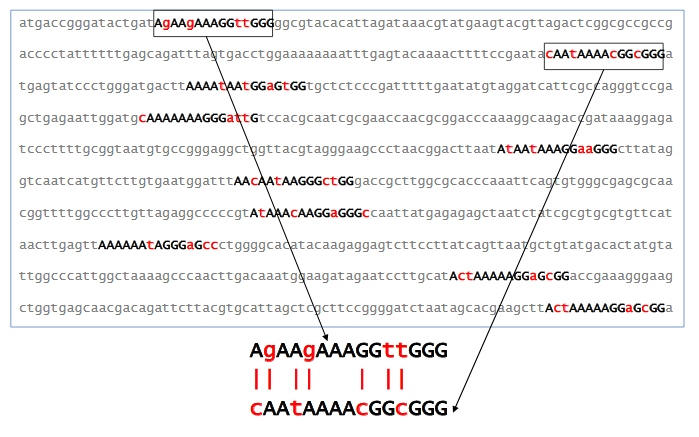
\includegraphics[width=0.9\textwidth]{poglavlja/2/slike/25.PNG}
\caption{Najsličniji k-grami u parovima niski - primer}
\label{slika: najslicniji kgrami}
\end{figure}

Zvuči predobro da bi bilo istinito? Pa možda ste i u pravu. 
Sličnost para niski je takođe određena brojem $d$. One se od kanonskog motiva mogu razlikovati na $d$ pozicija, što znači da se među sobom, mogu razlikovati na $2d$ pozicija.
Na malom izolovanom primeru, gde je bilo $d = 1$, zaista su slične niske isplivale kao dobri kandidati. Međutim, u praksi, sa (15,4)-motivima, broj dozvoljenih razlika je malo veći, čak 8. Kako izgledaju takvi parovi, prikazano je na slici \ref{slika: kgrami problem}, gde se jasno vidi koliko je to zaista mnogo i kako ove dve niske više i nisu tako slične.

\begin{figure}[h]
\centering
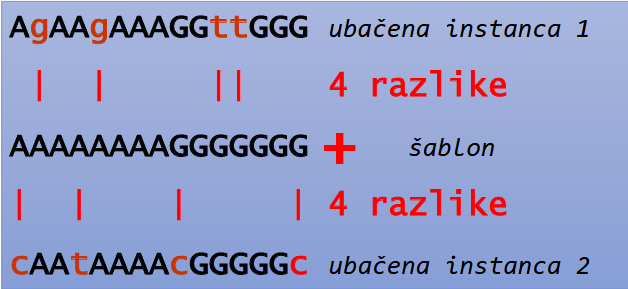
\includegraphics[width=0.7\textwidth]{poglavlja/2/slike/26.PNG}
\caption{Najsličniji k-grami u parovima niski - problem}
\label{slika: kgrami problem}
\end{figure}


Primer koji pokazuje koliko je ovo zaista loše rešenje je eksperiment rađen nad 10 slučajno generisanih niski iz $Dna$ dužine 600, sa ubačenim (15, 4) motivom. Pristupom pronalaženja parova niski iz $Dna$, pronađeno je nekoliko hiljada parova k-grama koji su se razlikovali na manje od 8 pozicija. Ovo sigurno nisu skrivene poruke, jer ih je previše. 

Da bismo ih pretražili u nekom smislenom redosledu, potrebno nam je da ih nekako rangiramo. Dakle, potreban nam je novi pristup.


\subsection{Matrice motiva}


Dosadašnje pretrage skupa $Dna$, nisu dale dobre rezultate. Pokušavali smo da ubrzamo pretragu na razne načine, ali bez puno uspeha. Možda je vreme da probamo da potpuno promenimo pristup, da mislimo izvan kutije. Pokušajmo da analiziramo jedan skup rešenja, i da malim koracima unazad dođemo do početnih uslova.

Pretpostavićemo da imamo neku kolekciju motiva i stavimo ih u matricu. Recimo da smo uradili jednom grubu pretragu i dobili neke rezultate. Da bismo olakšali komunikaciju, uvešćemo par pojmova koje ćemo koristiti u daljem tekstu.

\begin{itemize}
    \item Najpopularniji nukleotid u nekoj koloni matrice je onaj koji se pojavljuje najveći broj puta.
    \item Konsenzus niska predstavlja nisku koja se dobija nadovezivanjem najpopularnijih nukleotida iz svake kolone.
    \item Skor predstavlja broj nepopularnih simbola (onih koji nisu najpopularniji u svojoj koloni) u matrici.
\end{itemize}

Za lakše usvajanje, ilustrovani primer ovih pojmova prikazan je na slici \ref{slika: motivi skor}. Najpopularniji nukleotidi u svakoj koloni matrice motiva su napisani velikim slovima i boldovani. Oni su nadovezani u konsenzus nisku. Nepopularni simboli su napisani malim slovima, i njihov ukupan broj predstavlja skor.


\begin{figure}[h]
\centering
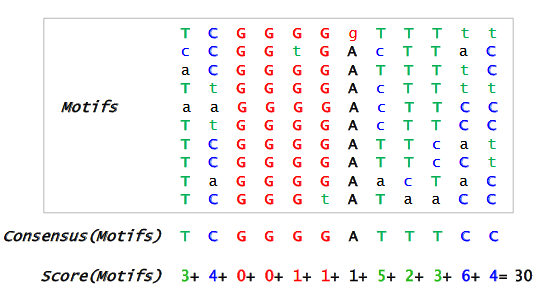
\includegraphics[width=0.9\textwidth]{poglavlja/2/slike/30.PNG}
\caption{Matrica motiva, konsenzus niska i skor}
\label{slika: motivi skor}
\end{figure}

Analizirajmo malo našu matricu rešenja. Ako bismo pretpostavili da su ovo instance nekog $(k,d)$ motiva, jasno, želeli bismo da one budu što sličnije, tj. da se razlikuju na što manje pozicija. Dakle, želimo da nam broj nepopularnih simbola bude što manji, odnosno želimo mali skor. Dakle, ako ovako postavimo problem, skor je zapravo "mera neuspeha", pa je ključ dobrog rešenja u minimizovanju ove veličine. Novi pojmovi, novi pristup i nova ideja, zahtevaju i malo drugačiju definiciju problema:

\begin{tcolorbox}
\textbf{Problem pronalaženja motiva:} Za dati skup niski iz $Dna$ naći skup k-grama (po jedan iz svake niske) sa minimalnim skorom među svim mogućim k-gramima iz datog skupa niski.\\
\textbf{Ulaz:} skup niski $Dna$ i ceo broj $k$.\\
\textbf{Izlaz:} skup k-grama $Motifs$, po jedan iz svake niske $Dna$, tako da je vrednost skora matrice $Motifs$ minimalna.
\end{tcolorbox}

Kada smo definisali problem, vreme je da krenemo da ga rešavamo.
Prvo što nam svakako pada na pamet je gruba sila. To je obično najjednostavniji algoritam, sa ne tako dobrom brzinom. Ali, ako on da zadovoljavajuću brzinu, nema potrebe komplikovati dalje, zar ne?

Dakle, krećemo redom. Uzimamo po jedan k-gram iz svake niske skupa $Dna$ i računamo skor. Tako redom obiđemo sve kombinacije k-grama, pamteći minimalni skor, i na kraju, proglasimo rešenjem onaj skup motiva sa najmanjim skorom.

Rešenje je dobro, pa hajde da pogledamo složenost. Neka je $t$ broj niski i $n$ dužina svake niske. Zaključujemo da je $(n-k+1)$ broj k-grama jedne niske, odnosno, 
$(n-k+1)^t$ broj kombinacija koje treba da proverimo. Vreme provere je konstantno (treba samo izračunati skor i ažurirati neku vrednost). Dakle, ukupna složenost je:
$(n-k+1)^t$. Eksponencijalna složenost svakako nije dobra, tako da zaključujemo da je ovaj algoritam prespor. Moramo ga nekako unaprediti.

Vratimo se na našu matricu motiva i pokušajmo da primetimo nešto što bi nam pomoglo da malo ubrzamo stvari. Pogledajmo primer dat na slici \ref{slika: motivi detaljnije}.

\begin{figure}[h]
\centering
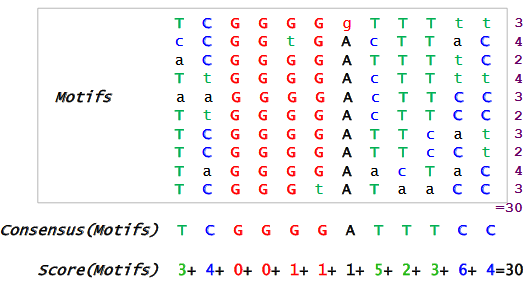
\includegraphics[width=0.9\textwidth]{poglavlja/2/slike/32.PNG}
\caption{Matrica motiva, konsenzus niska i skor - detaljnije}
\label{slika: motivi detaljnije}
\end{figure}


Izračunali smo skor po vrstama i primetili da je isti kao skor po kolonama. Da li je to slučajnost? Ispostavlja se da nije. Suština veličine skor leži u tome da broji nepopularne simbole. Nije važno kako ih prebrajamo, ako su svi na broju. 
Pojam brojanja definisaćemo na malo formalniji način. Definisaćemo veličinu koja se zove Hamingonovo rastojanje.

Hamingovo rastojanje između dve niske istih dužina predstavlja broj pozicija na kojima se one razlikuju. Npr. Hamingonovo rastojanje niski AACCTTGG i ATCCATGG je 2. Kada imamo Hamingovo rastojanje, možemo reći da je skor po kolonama suma Hamingovih rastojanja k-grama iz matrice od konsenzus niske. 


Vreme je da pokušamo da unapredimo naš algoritam. Želimo nekako da nađemo način da uradimo suprotno - da od konsenzus niske i niza $Dna$ dobijemo matricu $Motifs$. 
Koristićemo sledeće osobine koje smo primetili na matrici $Motifs$:
\begin{enumerate}
    \item Kako skor predstavlja sumu rastojanja od k-grama iz matrice do konsenzus niske, minimalni skor predstavlja minimizovanu sumu tih rastojanja.
    \item Kako je skor po kolononama i vrstama isti, možemo rastojanje računati i po vrstama. 
    Tako dolazimo do reforomulacije našeg problema, tj. njegovog ekvivalenta koji koristi naša nova zapažanja.
\end{enumerate}

Iskoristićemo ove osobine kako bismo još jednom predefinisali naš problem tako da odražava sliku iz novog pristupa.

\begin{tcolorbox}
\textbf{Problem pronalaženja motiva - reformulacija:} Naći k-gram $Pattern$ i skup k-grama $Motifs$ iz skupa niski $Dna$ koji minimizuju rastojanje između svih mogućim k-grama $Pattern$ i svih mogućih skupova k-grama $Motifs$.\\
\textbf{Ulaz:} skup niski iz $Dna$ i ceo broj $k$.\\
\textbf{Izlaz:} k-gram $Pattern$ i skup k-grama $Motifs$ iz skupa niski $Dna$ koji minimizuju $d(Pattern, Motifs)$.
\end{tcolorbox}

\noindent Ovo je ekvivalentno našem prethodnom problemu jer smo primetili da $d(Pattern, Motifs)$ predstavlja skor ukoliko je $Pattern$ konsenzus niska. Postavlja se pitanje da li smo ovim otežali naš problem. Ispostaviće se da nismo, jer ne moramo ispitivati sve skupove k-grama $Motifs$, već je dovoljno da iskoristimo problem niske medijane koji ispituje sve k-grame $Pattern$. 

\subsection{Problem niske medijane}
Prethodnom definicijom problema, nameće se zaključak da je sledeći prirodni korak proći kroz sve kombinacije skupa k-grama $Motifs$ i k-grama $Pattern$, kako bismo našli kombinaciju sa najmanjim rastojanjem. Međutim, videli smo i da algoritmi zasnovani na gruboj sili, tj. iscrpnoj pretrazi kombinacija u potrazi za pravom, vode ka ogromnoj složenosti i lošoj praktičnoj primeni. 

Zato ćemo ovaj put preskočiti taj korak i odmah krenuti da modifikujemo algoritam tako da dobijemo manju složenost. Primetićemo da imamo dve dimenzije pretrage (računarski bi to bile dve ugnježdene for petlje). Jedna je po svim k-gramima $Pattern$ a druga po skupovima $Motifs$. Jasno je da bi se složenost prepolovila (tj. korenovala) ako bismo imali samo jednu dimenziju. Zvuči neverovatno, ali je moguće, ako primetimo da nam unutrašnja for petlja nije potrebna, jer možemo uzeti cele niske umesto motiva. Tačnije, želimo da računamo rastojanje jednog k-grama od celog skupa $Dna$. Računanjem rastojanja od samih niski iz $Dna$ umesto od njihovih podniski dužine $k$, štedimo dosta vremena, a postižemo isti efekat. Međutim, da bismo to učinili, najpre moramo definisati nekoliko pojmova, na prvom mestu jer još uvek nismo rekli kako se računa rastojanje sem ako imamo dve niske i to iste dužine. Dakle, definisaćemo najpre sledeće pojmove: 

\begin{itemize}
    \item Hamingovo rastojanje izmedu dve niske različitih dužina predstavlja minimum Hamingovih rastojanja između kraće niske i svih podniski duže niske odgovarajuće dužine.
    \item Definišemo rastojanje između k-grama i skupa (dužih) niski kao sumu rastojanja između tog k-grama i svih niski iz skupa.
    \item Niska medijana za skup niski $Dna$ predstavlja onaj k-gram koji minimizuje rastojanje izmedu tog k-grama i skupa $Dna$ - $d(k-gram, Dna)$.
\end{itemize}

Novi pojmovi i nova ideja, prirodno vode i do nove definicije problema. Moramo dobro definisati problem koji rešavamo ako želimo da nas to dovede do dobrog algoritma za njegovo rešavanje.

\begin{tcolorbox}
\textbf{Problem niske medijane:} pronaći nisku medijanu.\\
\textbf{Ulaz:} skup niski $Dna$.\\
\textbf{Izlaz:} k-gram $k-mer$ koji minimuzuje rastojanje d($k-mer$, $Dna$).
\end{tcolorbox}

Sada imamo sav potreban alat da rešimo problem. Eliminišući jednu dimenziju, pretragu ćemo vršiti samo po svim mogućim kombinacijama k-grama $Pattern$ (njih $4^k$) i kao rezultat vratiti onaj k-gram koji ima najmanje ratojanje od skupa $Dna$. Ovaj algoritam se naziva \textit{MedianString} i prikazan je sledećim pseudokodom:

\begin{lstlisting}[escapeinside={(*}{*)}]
MedianString(Dna, k)
	best-k-mer (*$ \leftarrow $*) AAA...AA
    for each k-mer from AAA...AA to TTT...TT
        if d(k-mer, Dna) < d(best-k-mer, Dna)
            best-k-mer (*$ \leftarrow $*) k-mer
    return best-k-mer
\end{lstlisting}

Hajde da analiziramo složenost i vidimo da li smo zaista napredovali. Neka je $t$ dužina niza $Dna$ i $n$ dužina niske iz $Dna$. Tada nam je za izračunavanje rastojanja između jednog k-grama i jedne niske iz skupa $Dna$ potrebno $k \cdot (n-k+1)$ poređenja. Kako imamo $t$ niski, za izračunavanje rastojanja k-grama od skupa potrebno nam je $t \cdot k \cdot (n-k+1)$, odnosno približno $t \cdot k \cdot n$, jer je $n$ daleko veće od $k$ pa čini primarnu komponentu složenosti u $(n-k+1)$. Ceo taj postupak moramo izvršiti za svaki k-gram, odnosno $4^k$ puta, pa imamo, dakle, da ukupna složenost algoritma iznosi: $4^k \cdot n \cdot t \cdot k$. Primećujemo da je ovo dobar napredak u odnosu na $n^t \cdot k \cdot t$, ali i dalje imamo eksponencijalnu složenost. Dakle, iako je \textit{MedianString} algoritam mnogo brži od grube sile, za velike $k$ je i dalje prespor. 

\subsection{Probabilistički pristup}

\subsubsection{Uopšteno o pristupu}

Analizirali smo nekoliko determinističkih algoritama i videli da, iako uvek daju tačno rešenje, troše preveliku količinu vremena. Čak i najbolji među njima, \textit{MedianString}, imao je eksponencijalnu složenost. To nas navodi na razmišljanje da je možda ponovo došlo vreme da uradimo veliki zaokret u pristupu samom problemu i pokušamo da nađemo kompromis između tačnosti i utroška vremena. Algoritmi koji ovo omogućavaju se nazivaju probabilistički algoritmi. Oni daju tačno rešenje sa određenom verovatnoćom, ali za dosta manje vremena, i oni su naša sledeća stanica u potrazi za ubačenim motivima. Kao i svaki put kada menjamo pristup, upoznaćemo se najpre sa nekoliko osnovnih pojmova:
 
\begin{itemize}
    \item \textit{Count} matrica neke matrice motiva prikazuje koliko se puta koji nukleotid ponavlja u svakoj koloni matrice motiva.
    \item Profilna matrica neke matrice motiva prikazuje učestalost pojavljivanja nukleotida u svakoj koloni matrice motiva.
\end{itemize}

Ilustrovani primer ovih pojmova prikazan je na slici 2.9.

\begin{figure}[h]
\caption{\textit{Count} i profilna matrica}
\centering
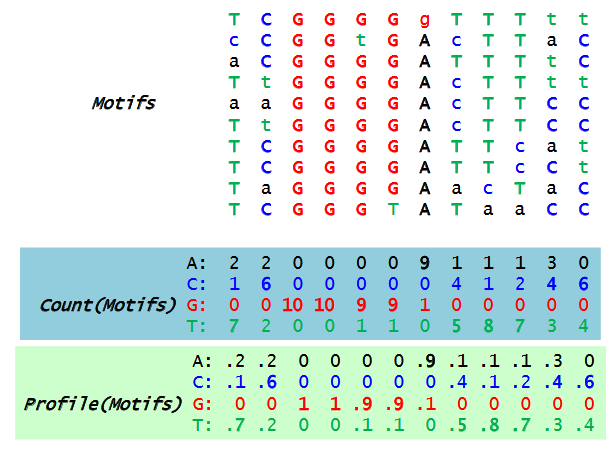
\includegraphics[width=0.9\textwidth]{poglavlja/2/slike/56.PNG}
\end{figure}

Osnovna ideja ovog pristupa može se ilustrovati bacanjem $k$ četvorostranih kockica sa otežanim stranama. Svaka kockica pretstavlja jednu poziciju u motivu dužine $k$, i na stranama ima simbole A, C, T i G. Strane kockica su otežane, tako da svaka strana pada sa onom verovatnoćom koja je zapisana u profilnoj matrici, u preseku kolone rednog broja pozicije u motivu i reda karaktera koji je na toj strani kockice. Na primer, ukoliko imamo profilnu matricu kao na slici 2.10, bacali bismo 6 četvorostranih kockica, gde bi recimo druga kockica bila otežana tako da simbol A pada sa verovatnoćom 7/8, simbol C sa verovatnoćom 0, simbol T sa verovatnoćom 1/8 i simbol G sa verovatnoćom 0. Naravno da u praksi ne možemo imati verovatnoću nula, ali sa našim zamišljenim kockicama, to je legitimna situacija. Zašto ovo nije dobro i kako se to popravlja, diskutovaćemo malo kasnije. 

Neka su redom pali karakteri: A, T, A, C, A i G. Verovatnoću podniske koju oni čine možemo izračunati na osnovu profilne matrice, pretpostavljajući da su bacanja nezavisni događaji. Dakle, pročitaćemo iz profilne matrice verovatnoću karaktera A na prvoj poziciji (1/2), verovatnoću karaktera T na drugoj (1/8), ... , i pomnožićemo sve te vrednosti. Proizvod verovatnoća iznosi 0.001602.

\begin{figure}[h]
\caption{Računanje verovatnoće k-grama}
\centering
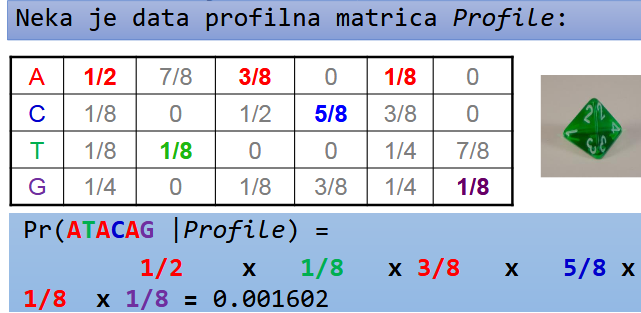
\includegraphics[width=0.5\textwidth]{poglavlja/2/slike/61.PNG}
\end{figure}

 Ako se setimo kako smo definisali matricu motiva, konsenzus nisku i profilnu matricu, lako možemo zaključiti da je ova verovatnoća zapravo verovatnoća da je niska ATACAG konsenzus niska. Sada nam same kockice više nisu potrebne, već možemo uzeti realne k-grame iz niski skupa $Dna$ i za njih računati. Na primer, za nisku CTATAAACCTTACAT iz nekog skupa $Dna$, možemo izračunati verovatnoće svih njenih podniski dužine 6 (rezultate možete videti na slici 2.11) i potražiti onaj sa najvećom verovatnoćom (u primeru sa slike 2.11 to je AAACCT). On je svakako dobar kandidat za ubačeni motiv. U ovome leži sama suština svih probabilističkih algoritama za traženje ubačenih motiva.

\begin{figure}[h]
\caption{Primer: najverovatniji 6-gram}
\centering
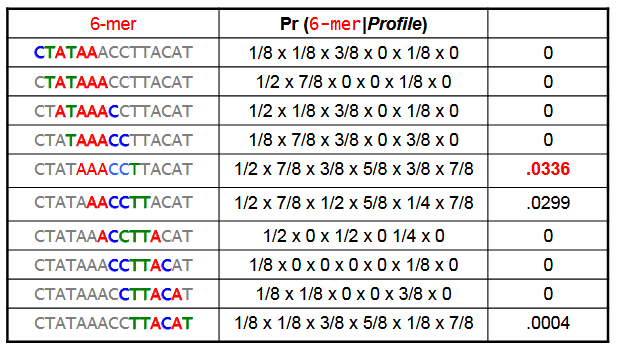
\includegraphics[width=0.8\textwidth]{poglavlja/2/slike/63-2.PNG}
\end{figure}

U daljem tekstu, predstavićemo nekoliko probabilističkih algoritama za rešavanje problema ubačenih motiva. Opisaćemo same algoritme, ali i diskutovati o njihovim dobrim i lošim stranama.

\noindent \textbf{Važna napomena}: Kao što smo već napomenuli, cenu malog vremena ovi algoritmi plaćaju tačnošću. Dakle, rešenje može malo odstupati od traženog. Zbog toga, za postizanje najbolje tačnosti, probabilističke algoritme treba pokretati više puta i uzeti najbolji rezultat.

\subsubsection{Algoritam \textit{Greedy motif search}}
Prvi algoritam koji ćemo predstaviti je pohlepni algoritam. Kao ulaz, on prima skup niski $Dna$, broj njegovih elemenata $t$ i dužinu ubačenog šablona $k$, a kao izlaz daje matricu ubačenih motiva $BestMotifs$. Suština algoritma leži u njegovom imenu: grabi k-mere iz jedne niske redom, na osnovu svakog od njih nađi najbolju matricu u koju se on uklapa, i uzmi onu koja ima najmanji skor.
Na početku $BestMotifs$ se inicijalizuje na $t$ podniski dužine $k$, od kojih svaka predstavlja prvih $k$ karakera jedne niske iz skupa $Dna$. Iterira se kroz prvu nisku skupa $Dna$, i iteracija ima onoliko koliko ima podniski dužine $k$ u njoj. U svakoj iteraciji, računa se po jedna matrica motiva. 

Građenje te matrice je jedan vid pohlepe ovog algoritma. Grabimo već izračunate vrednosti, kako bismo što bolje odredili sledeće. Prvi red čini tekuća podniska iteracije (podniska prve niske skupa $Dna$ koja počinje od karaktera na poziciji rednog broja iteracije). Za svaki sledeći red se pravi profilna matrica prethodno izračunatih redova i na osnovu nje računa najverovatnija podniska iz one niske skupa $Dna$, koja ima redni broj isti kao redni broj reda matrice koji računamo. Dakle, svaki sledeći motiv u matrici se sve lepše poklapa sa ostatkom matrice. Sledeći korak u iteraciji je da izračunamo skor i ako je manji, da ažuriramo vrednost $BestMotifs$. Dakle, ona matrica koja ima najmanji skor je tražena matrica $BestMotifs$. Sam algoritam ilustrovan je sledećim pseudokodom:


\begin{lstlisting}[escapeinside={(*}{*)}]
GreedyMotifSearch(Dna, k, t)
  BestMotifs (*$ \leftarrow $*) motif matrix formed by first k-mers in each string from Dna
  for each k-mer Motif in the first string from Dna
      Motif(*$_1 \leftarrow $*) Motif
      for i = 2 to t
        form Profile from motifs Motif(*$_1$*), ..., Motif(*$_{i-1}$*)
        Motif(*$_i  \leftarrow $*) Profile - most probable k-mer in the i-th string in Dna
      Motifs (*$ \leftarrow $*) (Motif(*$_1$*), ..., Motif(*$_t$*))
	  if Score(Motifs) < Score(BestMotifs)
        BestMotifs (*$ \leftarrow $*) Motifs
  return BestMotifs
\end{lstlisting}

\textit{GreedyMotifSearch} je brži od \textit{Median string} algoritma. Povoljan je i za veće $k$, ali cena toga je manja tačnost. Tačnost se može poboljšati primenom Laplasovog pravila, o kojem će biti nešto više reči malo kasnije.

\subsubsection{\textit{Randomized motif search}}
Posmatrajući algoritam \textit{GreedyMofifSearch}, možemo primetiti da nismo postigli pun potencijal po pitanju prelaska na probabilistički pristup. Broj iteracija je i dalje fiksan (zavisi isključivo od dužine niski iz skupa $Dna$ i dužine ubačenog motiva), a i sam njihov redosled je nametnut deterministički. Kako uvek krećemo od istog skupa motiva, i pratimo iste utabane korake, pokretanjem ovog algoritma više puta nećemo poboljšati ni tačnost ni vreme konvergencije. 

Hajde da pokušamo da potpuno izbacimo determinizam iz priče i da pustimo da izgled same niske $Dna$ i zakon verovatnoće igraju glavne uloge u konvergenciji algoritma. Prva ideja o poboljšanju probabilizma bi mogla biti vezana za sam početak algoritma. Hajde da umesto kretanja od početnih pozicija, krećemo od nekih nasumično odabranih. To sasvim sigurno donosi malo probabilizma u našu priču. Međutim, i dalje imamo iteriranje po jednoj od niski, što fiksira i broj iteracija i njihov redosled. To je ono što nam najviše i smeta. 

Na početku sekcije o probabilističkim algoritmima, naučili smo da pravimo profilnu matricu od matrice motiva, a u algoritmu \textit{GreedyMofifSearch} smo videli da je moguće i obrnuto. To je dobra ideja za osnovu iteracije. Od matrice motiva bismo mogli praviti profilnu matricu, a od profilne matrice ponovo matricu motiva. Ponavljanjem tog postupka, mogli bismo iterirati bez potrebe da se vezujemo za bilo kakav redosled podniski u nekoj od niski iz $Dna$. Ostalo je još da razmislimo kako bismo znali kada da stanemo. 

Pretpostavljajući da krećemo od neke nasumične matrice motiva sa lošim, tj. velikim skorom, pretpostavljajući da se krećemo ka dobrom rešenju koje ima mali skor, kao i da to činimo postepeno gradeći sve bolja, tj. verovatnija rešenja pomoću profilnih matrica, prirodno je da pomislimo da će se skor smanjivati iz iteracije u iteraciju. Dakle, iteriraćemo dokle god nam se skor smanjuje.

Ova ideja je zapravo osnova algoritma \textit{RandomizedMotifSearch}. Njegova suština leži u tome da u velikom broju iteracija ažuriramo matricu motiva i profilnu matricu tako da dobijamo sve verovatniji skup motiva, zaustavljajući se kada postignemo najniži skor. Ovaj algoritam je ilustrovan sledećim pseudokodom:

\begin{lstlisting}[escapeinside={(*}{*)}]
RandomizedMotifSearch(Dna, k, t)
  randomly select k-mers Motifs = (Motif(*$_1$*), ..., Motif(*$_t$*)) in each string from Dna
  bestMotifs (*$\leftarrow$*) Motifs
  while forever
    Profile (*$\leftarrow$*) Profile(Motifs)
    Motifs (*$\leftarrow$*) Motifs(Profile, Dna)
    if Score(Motifs) < Score(bestMotifs)
      bestMotifs (*$\leftarrow$*) Motifs
    else 
      return bestMotifs
\end{lstlisting}

Radi lakšeg razumevanja, hajde da ilustrujemo rad ovog algoritma na jednom primeru. Jedan takav, dosta uprošćen primer možemo videti na slici \ref{slika: randomized}. Prikazan je algoritam \textit{RandomizedMotifSearch} koji konvergira u jednoj iteraciji.

Neka je dat skup $Dna$ od 5 niski dužine 10 karaktera, sa ubačenim (4,1) motivom. Na slici \ref{slika: randomized} u gornjem levom uglu, prikazan je skup $Dna$, tako što su velikim slovima ispisani karakteri instanci ubacenog motiva: ACCT, ATGT, GCGT, ACGA i AGGT, crnom bojom označene mutacije na motivima, a plavom nemutirani karakteri motiva. 

Prvi korak jeste određivanje početne vrednosti matrice \textit{Motifs}. Odabraćemo slučajno 5 pozicija (u opsegu od 1 do 7) na kojima će početi 4-grami kojima ćemo inicijalizovati matricu \textit{Motifs}, i neka su to pozicije 7, 5, 1, 2 i 7. 4-grami koji počinju na ovim pozicijama: taac, GTct, ccgG, acta i AGGT, čine početnu matricu \textit{Motifs}. Sledeći korak jeste izgradnja profilne matrice na osnovu matrice \textit{Motifs}. Prebrojavanjem svakog karaktera u svakoj koloni matrice \textit{Motifs} možemo odrediti \textit{count} matricu, a zatim deljenjem svakog broja iz \textit{count} matrice sa brojem niski, tj. 5 u našem primeru, dobijamo profilnu matricu. 

Sada kada imamo profilnu matricu, možemo izračunati nove najverovatnije motive u niskama iz $Dna$, i ažurirati matricu \textit{Motifs}. Postupak računanja matrice motiva prikazan je na slici 2.12 u središnjem delu. Za svaku nisku iz skupa $Dna$, odredićemo verovatnoće svih njenih podniski, na osnovu profilne matrice, i iz svake niske odabrati po jednu koja ima najveću verovatnoću (na slici su prikazane ljubičastom bojom). 

Sledeći korak bi bio da ponovo napravimo profilnu matricu itd. Međutim, u našem primeru, vidimo da je to kraj. Dobili smo traženo rešenje. Treba napomenuti da je ovo veštački kreiran primer i da je u praksi broj iteracija dosta veći.

\begin{figure}[h]
\centering
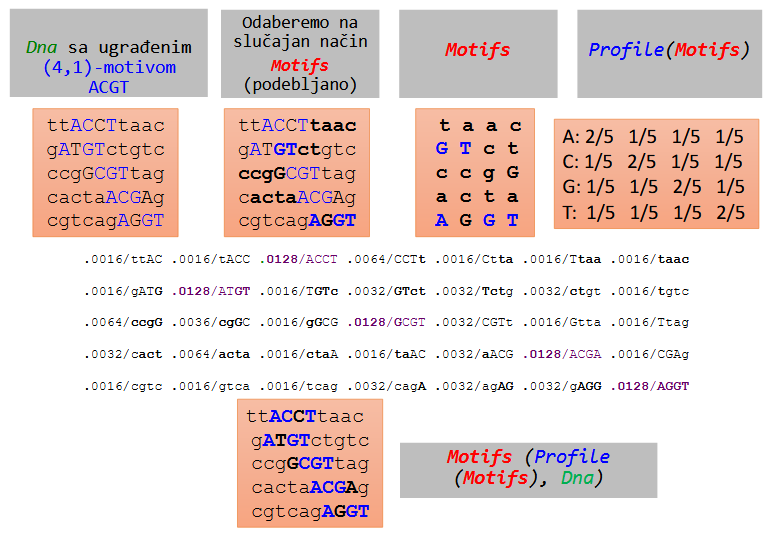
\includegraphics[width=0.8\textwidth]{poglavlja/2/slike/69.PNG}
\caption{Primer rada algoritma \textit{RandomizedMotifSearch}}
\label{slika: randomized}
\end{figure}


Velika prednost ovog algoritma je u nasumičnom izboru početnog skupa motiva, što nam omogućava da ga pokrećemo iznova i izaberemo najbolje rešenje.

\subsubsection{Gibsovo sempliranje}
Algoritam \textit{RandomizedMotifSearch} je dobar i efikasan, ali ima jednu malu manu. Matrica motiva se potpuno menja iz iteracije u iteraciju, što može dovesti do toga da se izmene i neki dobro izračunati redovi. To svakako ne želimo. Ako bismo u svakoj iteraciji menjali samo po jedan motiv iz matrice, tj. posle manjih izmena pravili novu profilnu matricu i proveravali skor, mogli bismo bolje da kontrolišemo to kvarenje već nameštenih motiva. Ova modifikacija algoritma \textit{RandomizedMotifSearch} se naziva Gibsovo sempliranje. Na prvi pogled deluje kao da povećava broj iteracija i usporava konvergenciju, ali to što su promene manje, nikako ne znači da su manje i efikasne. Ako idemo pravo sitnijim koracima, stižemo brže i lakše na cilj, nego ako krupnim koracima idemo levo-desno. 
Osnovna razlika Gibsovog sempliranja u odnosu na algoritam \textit{RandomizedMotifSearch} se nalazi u sadržaju iterativnog koraka. Umesto da od cele matrice motiva pravimo profilnu matricu i na osnovu nje ažuriramo celu matricu motiva, sada ćemo nasumično odabrati jedan motiv koji ćemo izbaciti, profilnu matricu praviti od ostatka matrice, a ažuriranje matrice motiva vršiti samo nad izbačenim redom u matrici. Postupak kreiranja same profilne matrice i ažuriranja motiva je potpuno isti kao u algoritmu \textit{RandomizedMotifSearch}. Umesto pseudokodom, ovaj put ćemo algoritam prikazati u koracima:

\begin{enumerate}
    \item Formirati \textit{Motifs} izborom jednog k-grama iz svake sekvence \textbf{na slučajan način}
    \item \textbf{Na slučajan način} odabrati jedan od k-grama i ukloniti ga iz \textit{Motifs} ; označimo sekvencu kojoj taj k-gram pripada sa \textit{RemovedSequence}
    \item Kreirati profilnu matricu \textit{Profile} od preostalih k-grama u \textit{Motifs}
    \item Za svaki k-gram iz \textit{RemovedSequence}, izračunati $Pr(k-mer|Profile)$ ; na taj način dobijamo $n-k+1$ verovatnoća: $p_1, p_2, ..., p_{n-k+1}$
    \item \textbf{Bacimo kockicu} sa $n-k+1$ strana kod koje je verovatnoća da će pasti na i-tu stranu proporcionalna verovatnoći $p_i$
    \item Odredimo k-gram iz sekvence \textit{RemovedSequence} kao onaj koji ima najveću verovatnoću i dodamo ga u \textit{Motifs}
    \item Ponavljamo korake 2-6
\end{enumerate}

Radi lakšeg razumevanja, prikazaćemo i ovaj algoritam na istom primeru kao i \textit{RandomizedMotifSearch}. Skica rada algoritma je prikazana na slici 2.13.

Neka je ponovo dat isti skup $Dna$ od 5 niski dužine 10 karaktera, sa ubačenim (4,1) motivom. Na slici \ref{slika: gibs} u gornjem levom uglu, prikazan je skup $Dna$, tako što su velikim slovima ispisani karakteri instanci ubačenog motiva: ACCT, ATGT, GCGT, ACGA i AGGT, crnom bojom označene mutacije na motivima, a plavom nemutirani karakteri motiva. Prvi korak je isti kao i u algoritmu \textit{RandomizedMotifSearch}: određivanje početne vrednosti matrice \textit{Motifs}. Odabraćemo slučajno 5 pozicija (u opsegu od 1 do 7) na kojima će početi 4-grami kojima ćemo inicijalizovati matricu \textit{Motifs}, i neka su to pozicije 7, 5, 1, 2 i 7. 4-grami koji počinju na ovim pozicijama: taac, GTct, ccgG, acta i AGGT, čine početnu matricu \textit{Motifs}. 

Sledeći korak jeste izbacivanje jednog motiva. Nasumičnim izborom jednog broja iz opsega (1,5), odredili smo motiv iz reda 3 da bude izbačen. Matrica \textit{Motifs} sada izgleda kao na slici \ref{slika: gibs} u gornjem desnom uglu. Naredni korak je izgradnja profilne matrice na osnovu matrice \textit{Motifs}. Ovaj postupak je takođe isti kao u algoritmu \textit{RandomizedMotifSearch}, samo je skup nad kojim radimo za jedan 4-gram manji. Prebrojavanjem svakog karaktera u svakoj koloni matrice \textit{Motifs} možemo odrediti \textit{count} matricu (slika \ref{slika: gibs} , centar-desno), a zatim deljenjem svakog broja iz \textit{count} matrice sa brojem motiva, tj. 4 u našem primeru, dobijamo profilnu matricu. 

Sada kada imamo profilnu matricu, možemo izračunati novi najverovatniji motiv u trećoj niski iz $Dna$, i ponovo popuniti treći red u matrici \textit{Motifs}. Vidimo da je podniska GCGT jedina sa pozitivnom verovatnoćom, pa samim tim i najvećom, tako da njome popunjavamo treći red matrice \textit{Motifs}. Sledeći korak bi bio da ponovo izbacimo nasumično odabrani motiv, napravimo profilnu matricu itd. Iterirali bismo sve dok skor ne prestane da se smanjuje. 


\begin{figure}[h]
\centering
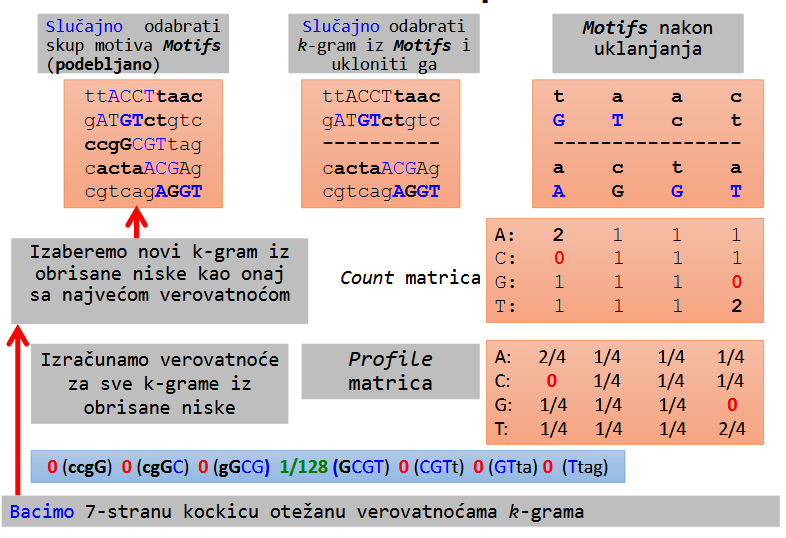
\includegraphics[width=0.8\textwidth]{poglavlja/2/slike/73.PNG}
\caption{Primer rada algoritma Gibsovo sempliranje}
\label{slika: gibs}
\end{figure}

Međutim, sada ćemo se ovde zaustaviti kako bismo primetili nešto mnogo važno. Kada smo računali verovatnoće podniski kandidata za zamenu trećeg motiva, dobili smo samo jednu ne-nula vrednost od 7. To nije dobro. Jedna nula u profilnoj matrici može anulirati verovatnoće koje su sve do množenja sa njom bile prilično velike. Zbog toga one nisu baš poželjne. Ako zastanemo malo i razmislimo, shvatićemo da nisu previše ni realne, tj. da ne odražavaju realnu verovatnoću, već da su u velikom broju slučajeva uzrokovane malim obimom skupa nad kojim računamo. Zbog toga, modifikicija nula u profilnoj matrici predstavlja vrlo dobru i poželjnu modifikaciju ovog algoritma, a ta modifikacija se sprovodi korišćenjem Laplasovog pravila.

Mala napomena: Setimo se da smo već pominjali Laplasovo pravilo kao dobro poboljšanje i \textit{GreedyMofifSearch} i \textit{RandomizedMotifSearch} algoritama. Zapravo, ovo je korisna modifikacija svakog algoritma koji se zasniva na računanju profilne matrice i korišćenju njenih vrednosti.

Pre nego pređemo na modifikaciju, naglasićemo još da se prednost Gibsovog algoritma ogleda u najmanjem skoru, kao i to da je mana ovog algoritma zaglavljivanje u lokalnom minimumu usled pretrage ograničenog skupa rešenja. 

\subsubsection{Laplasovo pravilo kao poboljšanje Gibsovog semplera}

Davne 1650. godine, Oliver Kromvel je napisao:
"Molim Vas, tako Vam Hrista, mislite da je moguće da grešite". 
Ovu izjavu, je uobličio Denis Lindli i nazvao Kromvelovo pravilo:
"Treba da ostavimo malu mogućnost da Sunce sutra neće izaći".
Nešto novija replika bi se mogla naći u seriji Smolvil i rečima Leksa Lutora: "Uvek ostavljam malu mogućnost da nisam u pravu. Tako me ništa ne može iznenaditi."
Suština Kromvelog pravila leži u tome da, ukoliko potpuno odbacimo mogućnost nekog događaja, sasvim sigurno ostavljamo mogućnost pogreške. Zbog toga, treba izbegavati verovatnoće 0 i 1.

Za poboljšanje Gibsovog semplera (zapravo se može primeniti na bilo koji algoritam koji računa profilnu matricu), izvršićemo malu modifikaciju algoritma primenom Laplasovog pravila. Primenjujemo Laplasovo a ne Kromvolevo pravilo, samo iz razloga notacije i matematičkog zapisa. Laplasovo pravilo je samo preciznija (matematička) formulacija Kromvelovog pravila, sa istom suštinom. 

\begin{tcolorbox}
\textbf{Laplasovo pravilo:} U malim skupovima podataka uvek postoji šansa da se događaj koji je moguć ne desi. Slučajni algoritmi uvode pseudovrednosti koje povećavaju verovatnoće retkih događaja i eliminišu frekvencije jednake nuli zabeležene na osnovu iskustva.
\end{tcolorbox}

\indent Suština Laplasovog pravila leži u tome da, ukoliko znamo da se događaj nekada u prošlosti desio, on ne može imati verovatnoću nula. Stoga u računanje, pored vrednosti dobijenih u našem eksperimentu, ubacujemo i dve pseudovrednosti: događaj se desio i događaj se nije desio. \\

\noindent Računanje uslovne verovatnoće bez primene Laplasovog pravila bi bilo:
\begin{tcolorbox}
Ako su $X_1, ..., X_{n+1}$ uslovno nezavisne slucajne logičke promenljive (neuspeh 0, uspeh 1), tada: $Pr(X_{n+1}=1|X_1+...+X_n=s)=s/n$
\end{tcolorbox}

\noindent Računanje uslovne verovatnoće sa primenom Laplasovog pravila bi bilo:
\begin{tcolorbox}
Ako su $X_1, ..., X_{n+1}$ uslovno nezavisne slučajne logičke promenljive (neuspeh 0, uspeh 1), tada: $Pr(X_{n+1}=1|X_1+...+X_n=s)=(s+1)/(n+2)$
\end{tcolorbox}

Modifikacija Gibsovog algoritma primenom Laplasovog pravila je sadržana u dva mala koraka. Prva izmena je u okviru računanja \textit{count} matrice, gde se vrednost svakog polja uvećava za 1. To je zapravo pseudovrednost: događaj se desio. Pod događaj, podrazumeva se pojava određenog karaktera na određenoj poziciji u matrici motiva. Druga izmena je u okviru računanja profilne matrice, zato što \textit{count} matrica izgleda nešto drukčije. 

Modifikaciju Gibsovog algoritma ćemo prikazati samo na primeru, jer je skup koraka u suštini isti i ne prikazuje najbolje samu modifikaciju. Koristićemo isti primer na kome smo već demonstrirali rad Gibsovog semplera. Na slici \ref{slika: gibs i laplas} prkazan je rad modifikovanog Gibsovog semplera. Možemo primetiti da \textit{count} i profilna matrica izgledaju nešto drukčije (dodate su pseudovrednosti), kao i da je rezultat 7 ne-nula verovatnoća.

\begin{figure}[h]
\centering
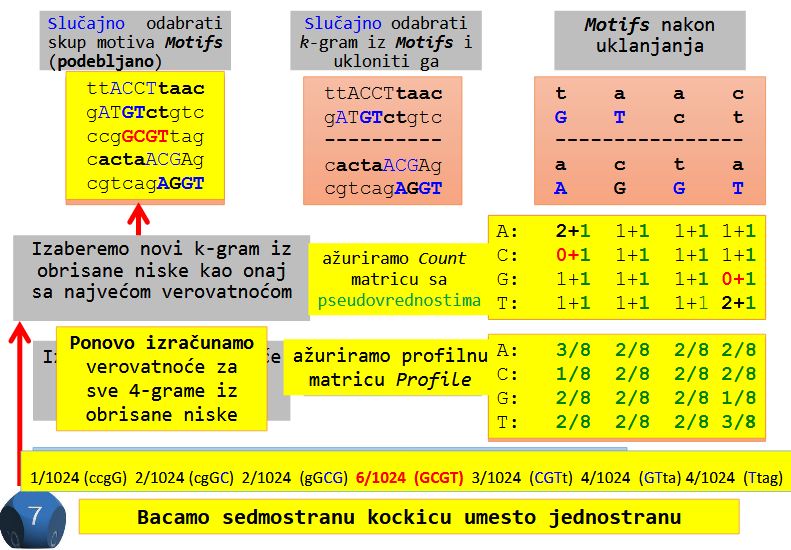
\includegraphics[width=0.7\textwidth]{poglavlja/2/slike/84.PNG}
\caption{Primer rada Gibsovog sempliranja sa primenom Laplasovog pravila}
\label{slika: gibs i laplas}
\end{figure}

\subsection{Koji princip odabrati?}
Odgovor na ovo pitanje je - nema pravila. Nekada će se bolje pokazati jedan, a nekada drugi. Najbolje je da isprobamo više algoritama i vidimo koji se najbolje ponaša u našem slučaju. Možemo koristiti već zapažene prednosti i mane u izboru, kao na primer biranje \textit{Median string} algoritma pri malim vrednostima $k$, ali isprobavanje je ipak najpouzdaniji pristup.

